
%%%%%%%%%%%%%%%%%%%%%%% file typeinst.tex %%%%%%%%%%%%%%%%%%%%%%%%%
%
% This is the LaTeX source for the instructions to authors using
% the LaTeX document class 'llncs.cls' for contributions to
% the Lecture Notes in Computer Sciences series.
% http://www.springer.com/lncs       Springer Heidelberg 2006/05/04
%
% It may be used as a template for your own input - copy it
% to a new file with a new name and use it as the basis
% for your article.
%
% NB: the document class 'llncs' has its own and detailed documentation, see
% ftp://ftp.springer.de/data/pubftp/pub/tex/latex/llncs/latex2e/llncsdoc.pdf
%
%%%%%%%%%%%%%%%%%%%%%%%%%%%%%%%%%%%%%%%%%%%%%%%%%%%%%%%%%%%%%%%%%%%


\documentclass[runningheads,a4paper]{llncs}
\usepackage[ngerman]{babel}
\usepackage[T1]{fontenc}% wichtig für Trennung von Wörtern mit Umlauten
\usepackage{microtype}% verbesserter Randausgleich
\usepackage[utf8]{inputenc}
\usepackage{amssymb}
\setcounter{tocdepth}{3}
\usepackage{graphicx}
\usepackage{amsmath}
\usepackage{amssymb}

\usepackage{subfigure}
\usepackage{eurosym}

\usepackage{url}    
\usepackage[
    backend=biber,
    style=authoryear-icomp,
    sortlocale=de_DE,
    url=false, 
    doi=true,
    eprint=false
]{biblatex}
\addbibresource{eakte.bib}
\newcommand{\keywords}[1]{\par\addvspace\baselineskip
\noindent\keywordname\enspace\ignorespaces#1}

\begin{document}

\mainmatter  % start of an individual contribution

% first the title is needed
\title{Rechtliche und technische Aspekte der E-Akte in der Anwaltschaft}

% a short form should be given in case it is too long for the running head
\titlerunning{Aspekte der E-Akte in der Anwaltschaft}

% the name(s) of the author(s) follow(s) next
%
% NB: Chinese authors should write their first names(s) in front of
% their surnames. This ensures that the names appear correctly in
% the running heads and the author index.
%
\author{Johannes Lahann}%
%
\authorrunning{}
% (feature abused for this document to repeat the title also on left hand pages)

% the affiliations are given next; don't give your e-mail address
% unless you accept that it will be published
\institute{}

%
% NB: a more complex sample for affiliations and the mapping to the
% corresponding authors can be found in the file "llncs.dem"
% (search for the string "\mainmatter" where a contribution starts).
% "llncs.dem" accompanies the document class "llncs.cls".
%

\toctitle{Lecture Notes in Computer Science}
\tocauthor{Authors' Instructions}
\maketitle

\begin{abstract}


Das Gesetz zur Förderung des elektronischen Rechtsverkehrs mit den Gerichten vom 10.10.2013 erlaubt ab 01.01.2022 als Kommunikationsweg zu den Gerichten einzig den elektronischen Rechtsverkehr.

Für Rechtsanwälte bedeutet dies, dass Schriftsätze bei Gericht ausschließlich auf elektronischem Weg eingereicht werden dürfen. Ein erster Schritt beinhaltet die Einführung besonderer elektronischer Anwaltspostfächer durch die Bundesrechtsanwaltskammer, welche bereits ab dem 01.01.2016 genutzt werden sollen.

Der Beitrag befasst sich mit den daraus resultierenden Konsequenzen sowohl im Bereich der Kommunikationswege zwischen Anwälten und Gerichten als auch in der internen Organisation einer Anwaltskanzlei. Insbesondere sollen die rechtlichen Anforderungen und die daraus ableitbaren technischen Herausforderungen diskutiert und Lösungsansätze erarbeitet werden.
\keywords{ERV-Gesetz, Elektronische Akte, Besonderes elektronisches Anwaltspostfach, Sicherheit und Datenschutz, Integrität, Authentizierung, Autorisierung, Digitale Signaturen, Anwaltskanzlei, Gericht}
\end{abstract}

\section{Einleitung}

\subsection{Motivation}
Der digitale Fortschritt ist in der heutigen Welt nicht mehr wegzudenken. Dies beinhaltet auch die Digitalisierung innerhalb der Justiz. Durch das Gesetz zur Förderung des elektronischen Rechtsverkehrs mit den Gerichten vom 10.10.2013 erhält diese Entwicklung einen weiteren deutlichen Schub. In naher Zukunft soll die Kommunikation mit den Gerichten ausschließlich elektronisch ablaufen. Dazu soll bis zum 01.01.2016 ein besonderes elektronisches Anwaltspostfach eingeführt werden und bis zum 01.01.2022 soll die Übermittlung der vorbereitenden Schriftsätze sowie deren Anlagen zwischen Rechtsanwälten und den Gerichten nur noch auf elektronischen Wege stattfinden. 
Damit das Gesetz erfolgreich umgesetzt werden kann, bedarf es Anpassungen sowohl in den Kommunikationswegen zwischen Anwälten und Gerichten als auch in der internen Organisation in der Anwaltskanzlei. Insbesondere ist eine Wechsel auf eine digitale Datenverwaltung zwar nicht rechtlich gefordert, aber allein aus Effizienzgründen sinnvoll. Dabei ergeben sich technische und rechtliche Bedingungen, welche miteinbezogen werden müssen.  

\subsection{Zielstellung}
Das Ziel dieser Arbeit ist die Ausarbeitung der technischen und rechtlichen Aspekte der elektronischen Akte innerhalb der Anwaltskanzlei. Insbesondere sollen:
\begin{itemize}
\item die sich neu ergebenen rechtlichen Herausforderungen während der Kommunikation zwischen Anwalt und Client sowie Anwalt und Gericht als auch innerhalb der internen Organisation definiert werden.  Dabei soll vor allem das neue elektronische Anwaltspostfach näher beleuchtet werden.
\item aus den rechtlichen Aspekten, die technischen Problemstellungen abgeleitet und unter zu Hilfenahme aktueller Literatur verschiedene Lösungsansätze herausgefiltert werden.
\item  Vorschläge gegeben werden, wie durch Einführung der E-Akte die Arbeitsabläufe in der Anwaltschaft und mit dem Mandanten sowie vor Gericht beschleunigt werden können.
\end{itemize} 
\subsection{Gliederung}
Im ersten Teil der Arbeit (Kapitel 2) wird die aktuelle Gesetzeslage bzgl. des Gesetz zur Förderung des elektronischen Rechtsverkehrs mit den Gerichten vorgestellt. Dabei werden insbesondere die Begriffe  Elektronisches Übermittlungswege, Elektronische Dokumente, Elektronische Formulare sowie das Elektronische Schutzschriftenregister näher erörtert. Kapitel 3 beschreibt die Auswirkungen des Gesetzes auf die Anwaltskanzleien und die daraus resultierenden technischen Herausforderungen. In Kapitel 4 wird der technische Hintergrund geschaffen, um die in Kapitel 3 erörterten Anforderungen technisch zu diskutieren. Dabei werden unter anderem aktuelle Verfahren zur Authentifizierung, Autorisierung und zur Erstellen von digitalen Signaturen vorgestellt. Kapitel 5-7 befassen sich mit der visuellen und technischen Umsetzung des Anwaltspostfachs(folgt eine kurze Erklärung was genau).  Abschließend werden in Kapitel 6 die Ergebnisse der vorherigen Kapitel zusammengefasst und Ergänzungen sowie ein Ausblick gegeben. 



\section{Gesetz zur Förderung des elektronischen Rechtsverkehrs mit den Gerichten}
Das Gesetz zur Förderung des elektronischen Rechtsverkehrs mit den Gerichten ändert die Prozessordnungen und Verfahrensgesetze für die Gerichte grundlegend. Bisher konnten die Länder selbst über die Einführung der elektronischen Verordnungswege entscheiden. Dies wird durch eine bundesweit eintretende Regelung am 01.01.2022 ersetzt, die ausschließlich elektronischen Kommunikationswege für Anwälte und Behörden zu den Gerichten erlaubt. Gleichzeitig wurden an mehreren Stellen Vorschriften zur Barrierefreiheit in die Gesetze eingefügt. In diesem Kapitel werden die wesentlichen gesetzlichen Änderungen vorgestellt. Dazu werden als Quellen im wesentlichen \textcite{Gesetzfoerderungrechtsverkehr}\footfullcite{Gesetzfoerderungrechtsverkehr} und \textcite{carstens2015grundlagen}\footfullcite{carstens2015grundlagen} herangezogen.
\subsection{Elektronisches Anwaltspostfach, § 31a BRAO}
Nach § 31a der Bundesrechtsanwaltordnung (BRAO) müssen Rechtsanwälte ab dem 1. Januar 2016 für die Gerichte über ein besonderes elektronisches Anwaltpostfach erreichbar sein. Die besonderen elektronischen Anwaltspostfächer werden von der Bundesrechtsanwaltskammer für die Rechtsanwälte eingerichtet. Eine detaillierte Beschreibung des elektronischen Anwaltspostfach folgt in Kapitel 5 bis Kapitel 7.
\subsection{Elektronische Übermittlungswege, § 130a ZPO}
Nach § 130a der Zivilprozessordnung (ZPO) müssen vorbereitende Schriftsätze und deren Anlagen, schriftlich einzureichende Anträge und Erklärungen der Parteien sowie schriftlich einzureichende Auskünfte, Aussagen, Gutachten, Übersetzungen und Erklärungen Dritter ab dem 01.01.2018 flächendeckend als elektronisches Dokument bei Gericht eingereicht werden können. Während elektronische Dokumente an das Gericht bisher mit einer qualifizierten elektronischen Signatur nach dem Signaturgesetz versehen sein müssen, wird es zukünftig möglich sein, elektronische Dokumente auch ohne qualifizierte elektronische Signatur zu übermitteln, wenn hierfür einer der nachfolgenden, vom Gesetzgeber im Hinblick auf die die Authentizität und die Integrität des übermittelten elektronischen Dokuments als sicher bezeichneten Übermittlungswege genutzt werden. Als sichere Übermittlungswege benennt das Gesetz in § 130a Abs. 4 ZPO :
\begin{enumerate}
\item das Postfach und Versanddienst eines De-Mail Kontos
\item die Nutzung des elektronischen Anwaltspostfach 
\item den Übermittlungsweg zwischen einem hierfür eingerichteten elektronischen Postfach einer Behörde und der elektronischen Poststelle des Gerichts 
\item sonstige bundeseinheitliche Kommunikationswege, die durch Rechtsverordnung festgelegt werden.
\end{enumerate} 
\subsection{Elektronische Dokumente, § 174 ZPO}
Mit der flächendeckenden Einführung des elektronisches Rechtsverkehrs wird es möglich werden, sowohl die Schriftsätze der Verfahrensbeteiligten und Erklärungen Dritter als auch gerichtliche Dokumente als elektronisches Dokument zu übermitteln. Nach § 174 Abs. 3 Satz 4 ZPO werden Rechtsanwälte und andere Prozessbevollmächtigte zudem verpflichtet, ab dem 01.01.2018 einen sicheren Zugang im Sinne des § 130a ABS.4 ZPO für Zustellungen elektronischer Dokumente durch das Gericht zu eröffnen. Daher werden elektronische Dokumente des Gerichts die bisherigen Papierdokumente zunehmend ersetzen. § 191a ABs. 3 Satz 1 GVG sieht vor, dass die Texte barrierefrei zugänglich und nutzbar sein müssen. Daneben können auch Fotos und Skizzen beigefügt werden. Für elektronische Dokumente, die an das Gericht übermittelt werden, sieht § 130a Abs.2 Satz 1 ZPO vor, dass sie für die Bearbeitung durch das Gericht geeignet sein müssen. Die technischen Rahmenbedingungen werden durch die Rechtsverordnung festgelegt. Insbesondere soll eine Bearbeitungs- und Suchfunktion der elektronischen Dokumente bereitgestellt werden. Daher soll die Übermittlung elektronischer Dokumente als Scans bzw. Bilder auf zu Beweiszwecken eingescannte Urkunden, Nachweise und Belege begrenzt werden. 
\subsection{Elektronische Formulare, § 130c ZPO}
Nach § 130c ZPO kann das Bundesministerium der Justiz für die elektronische Kommunikation mit den Gerichten ab dem 1. Juli 2014 durch Rechtsverordnung elektronische Formulare einführen. Die Rechtsverordnung kann bestimmen, dass die in den Formularen enthaltenen Angaben ganz oder teilweise in strukturierter maschinenlesbarer Form zu übermitteln sind. Die Formulare sind auf einer in der Rechtsverordnung zu bestimmenden Kommunikationsplattform im Internet zur Nutzung bereitzustellen.  Die Rechtsverordnung kann bestimmen, dass eine Identifikation des Formularverwenders abweichend von § 130 a Absatz 3 ZPO auch durch Nutzung des elektronischen Identitätsnachweises nach § 18 des Personalausweisgesetzes erfolgen kann. Elektronische Formulare sind nach § 191a Abs. 3 Satz 1 bzw. Satz 3 GVG blinden oder sehbehinderten Personen barrierefrei zugänglich und nutzbar zu machen.
\subsection{Elektronisches Schutzschriftenregister, § 945a Abs. 1 ZPO}
Die Vorschrift des § 945a Abs. 1 ZPO sieht vor, dass die Länder ein zentrales länderübergreifendes elektronisches Register für Schutzschriften führen. Schutzschriften sind vorbeugende Verteidigungsschriftsätze gegen erwartete Anträge auf Arrest oder einstweilige Verfügung . Hierzu regelt die Verordnungsermächtigung in § 945 b ZPO, dass das Bundesministerium der Justiz durch Rechtsverordnung die näheren Bestimmungen über die Barrierefreiheit festlegt.
Auch dieses neue Regelung sieht ab 1.1.2017 eine Nutzungspflicht für Anwälte vor. Nach § 49c BRAO ist der Rechtsanwalt verpflichtet Register ausschließlich über das elektronische Schutzschriftenregister einzureichen.

\section{Auswirkungen der elektronischen Akte auf die Anwaltskanzlei}
In diesem Kapitel werden die Auswirkungen des Gesetzes auf die Anwaltskanzleien und die daraus resultierenden technischen Herausforderungen beschrieben. Dazu wird zuerst anhand eines typischen Ablaufs in einer Kanzlei kurz dargestellt, welche Interaktionen mit einer Akte während einer anwaltlichen Rechtsberatung erfolgen. Darauf folgend werden rechtliche Anforderungen definiert, die an den Rechtsverkehr und die elektronische Dokumente gestellt werden müssen.
\subsection{Anwaltliche Rechtsberatung}
Zunächst wird – nachdem das Mandatsverhältnis begründet wurde – eine Akte angelegt, sei es physisch oder elektronisch oder beides. Bei der Aktenanlage werden der Akte bereits bestimmte Daten zugewiesen, nämlich insbesondere Name und Anschrift des Mandanten und des Gegners, Kontaktmöglichkeiten, Bezeichnung der Angelegenheit, Verfahrensstand, Art der Beratung (außergerichtlich, gerichtlich 1. Instand, 2. Instanz) sowie ggf. kanzleiinterne Daten wie zum Beispiel Name des Mandatsführers, des Sachbearbeiters und Informationen zu Abrechnung (nach Vergütungsvereinbarung, nach Gebührenstreitwert RVG oder Übernahme Kosten Rechtschutzversicherung bzw. Prozesskostenhilfe). Insbesondere die Adressdaten des Mandanten und des Gegners sind relevant, da es erforderlich wird, in einem frühen Stadium eine Prüfung durchzuführen, ob der Gegner in dieser Angelegenheit bereits durch einen Rechtsanwalt der Kanzlei vertreten wurde oder noch vertreten wird. In diesem Fall, kann das Mandat nicht übernommen werden, da die Gefahr eines Interessenkonflikts besteht. Die Aktenanlage erfolgt üblicherweise durch das Sekretariat auf Veranlassung durch den sachbearbeitenden Rechtsanwalt.
 
Nach erfolgter Aktenanlage wird die Akte dem Rechtsanwalt zur Bearbeitung vorgelegt. Dieser prüft Sachverhalt und Rechtslage und wird je nach Ergebnis der Prüfung entsprechendes veranlassen, also meist Schriftsätze an den Mandanten, den Gegner oder im Falle eines Gerichtsverfahrens an das Gericht abdiktieren, die sodann im Sekretariat geschrieben werden oder diese selbst verfassen. Von jedem Schriftsatz an den Gegner oder das Gericht erhält der eigene Mandant eine Abschrift. Die Kommunikation der Rechtsanwälte mit den Mandanten erfolgt im Regelfall über Briefverkehr. Nach Absprache ist auch die Nutzung von Emails denkbar. In beiden Fällen besteht ein nicht zu unterschätzender Aufwand in der Formatierung der Schriftsätze, des Einfügens der Adressen der Beteiligten und in der Formulierung des korrekten Rubrums (Bezeichnung Mandant und Gegner) bei Schriftsätzen in einem Gerichtsverfahren.
 
Bei der Aktenführung wird üblicherweise zwischen Gerichts- und Handakte unterschieden. Während die Gerichtsakte allen Schriftverkehr mit dem Gericht enthalten sollte, enthält die Handakte die Kommunikation mit dem Mandanten, sowie Aufzeichnungen, Entwürfe und interne Prüfergebnisse des Rechtsanwalts. Das Führen der Akte, also die Zuordnung der Unterlagen zu Gerichts- oder Handakte erledigt meist der Rechtsanwalt. Der Unterschied besteht darin, dass der Rechtsanwalt die eigenen Aufzeichnungen und Prüfungen bei Beendigung des Mandatsverhältnisses zurückhalten darf bis sein Honorar vollständig gezahlt wurde. Außerdem ist es hilfreich bei der Prozessführung, wenn die eigene Akte möglichst vollständig der Akte, die dem Gericht vorliegt, entspricht.
 
Sofern in einer laufenden Angelegenheit Post in der Kanzlei eingeht, wird die Post von dem Sekretariat gesichtet und der jeweiligen Akte zugeordnet und sodann dem Sachbearbeiter vorgelegt. Wenn eine elektronische Akte verwendet wird, wird vor der Vorlage beim Sachbearbeiter der Posteingang eingescannt. Schriftsätze die von Gericht oder dem Gegner kommen, werden dem Mandanten zur Kenntnis übersandt.

\subsection{Anforderungen}
Durch die Einführung des elektronischen Rechtsverkehrs am 01.01.2022 wird die Kommunikation zwischen Anwalt und Gericht ausschließlich auf elektronischem Wege möglich sein. Für die interne Organisation - insbesondere die interne Aktenverwaltung - sowie die Kommunikation zwischen Anwalt und Mandant gibt es keine rechtliche Verordnung. Trotzdem ist aus Effizienzgründen sinnvoll, langfristig komplett auf elektronische Datenspeicherung sowie Kommunikation umzusteigen. Zudem bisher bereits viele Kanzleien, sowohl eine digitale Aktensicherung sowie in Papierform verwenden, und auch die Kommunikation auf elektronischen Wege, wie z.B. per Email oder via direkten Zugriff auf ein digitales Laufwerk erfolgt. 
\subsubsection{elektronische Aktenführung}\hspace*{\fill} \\
Für die elektronische Aktenverwaltung in einer Kanzlei lassen sich Sicherheitskriterien herleiten, entsprechend der Anforderungen an die E-Akte nach \citeauthor{eakten-anforderungen}\footfullcite{eakten-anforderungen}.
\textcite{eakten-anforderungen} wählen die klassischen Schutzziele der It-Sicherheit als Grundlage und konkretisieren diese für den Anwendungsfall der Zivilprozessakte.
\begin{itemize}
\item \textit{Vertraulichkeit:}
Nur Menschen mit den notwendigen Berechtigungen dürfen Zugriff auf die Information erhalten. Dies beinhaltet sowohl die Einsicht einzelner Dokumente als auch die Übersicht über die vorhandenen Informationen. Berechtigungen müssen sich je nach Aktenbestand unterscheiden und können sich über einen Zeitraum ändern. Außerdem muss gegebenenfalls zwischen Lese und Bearbeitungsrechten unterschieden werden.
\item \textit{Authentizität und Integrität:}
Der Autor eines Dokumentes muss klar erkennbar sein. Dabei darf es nicht möglich sein sich als andere Person auszugeben. Ein Dokument darf nur verändert werden, wenn die notwendigen Berechtigungen vorliegen. 
\item \textit{Revisionssicherheit:}
Falls ein Dokument über einen Zeitraum verändert wurde, muss die Historie der Veränderungen einsehbar sein. Dabei sollte für jede Änderung Zeitpunkt und Autor der Änderung vorliegen. Des weiteren sollten vergangene Änderungen gegebenenfalls rückgängig gemacht werden können.
\item \textit{Verbindlichkeit:}
Wie im vorigen Abstritt beschrieben muss der Autor eines Dokumentes zu jedem Zeitpunkt eindeutig identifiziert werden können. Daraus folgt, dass es nicht möglich ist die Autorenschaft eines Dokumentes abzustreiten.
\item \textit{Verfügbarkeit:}
So wie die notwendigen Berechtigungen vorliegen, sollte ein Dokument zu jedem Zeitpunkt einsehbar sein.
\end{itemize}
Sie erweitern die oben genannten Schutzziele um:
\begin{itemize}
\item \textit{Schutz personenbezogener Daten:}
Trotz der gegebenen Informationen soll die elektronische Akte nicht genutzt werden können um die Arbeitszeiten zu überwachen. So sollen z.B. die Änderungszeitpunkte der Dokumente durch die Richter verborgen bleiben. Diese Anforderung steht im direkten Konflikt mit der Revisionssicherheit.
\item \textit{Langzeitarchivierung:}
Die Ziele müssen von der erstmaligen Anlage der E-Akte über den rechtskräftigen Abschluss hinaus erreicht werden.
\end{itemize}
\citeauthor{rechtsvekehranwaltskanzlei}\footfullcite{rechtsvekehranwaltskanzlei} benennt weitere Anforderungen an elektronische Dokumente innerhalb der Anwaltskanzlei:
\begin{itemize}
\item \textit{Erzeugung:}
Jede Kanzlei muss bis zum Inkrafttreten der Nutzungspflicht am 1. Januar 2022 Schriftsätze Anlagen und sonstige Dokumente in elektronischer Form zu erstellen. Aus Sicherheitsgründen (siehe Anforderungen Revisionssicherheit, Authentizität \& Integrität) ist es empfehlenswert die Dokumente im pdf-Format einzureichen.  Papierdokumente von Mandanten können eingescannt und in PDF-Form gespeichert werden
\item \textit{Signatur:}
Signatur durch besonderes elektronisches Anwaltspostfach
Dateisignatur am Dokument selbst angebracht
Container-Signatur
\item \textit{Versand:}
Der Versand elektronischer Dokumente an das Gericht ist normalerweise an bestimmte Fristen gebunden.
Die Führung der Akten in der Kanzlei kann sowohl elektronisch als auch in Papierform erfolgen und ist dem Anwalt freigestellt. Die elektronische Authentifizierung eines einzureichendem Dokumentes muss zwingend durch den Anwalt passieren. (vgl. Zugangsberechtigung). Nach der Authentifizierung kann der Versand von einen anderen Kanzleimitarbeiter übernommen werden. Die Übermittlung des Dokuments muss, wie in Abschnitt elektronische Übermittlungswege beschrieben, auf einen sicheren Übermittlungsweg erfolgen. Dies ist z.B. durch die Nutzung des elektronischen Anwaltspostfach gegeben.
\end{itemize}
	  

\subsubsection{Besonderes elektronisches Anwaltspostfach § 31a Brao}\hspace*{\fill} \\
Für die sichere elektronische Kommunikation zwischen Anwälten und Gerichten soll ab dem 01.01.2016 das besondere elektronische Anwaltspostfach bereitgestellt werden. \textcite{rechtsvekehranwaltskanzlei} definiert die hierzu folgenden Anforderungen:
\begin{itemize}
\item \textit{Erreichbarkeit:}
Das elektronische Anwaltspostfach muss für jeden Rechtsanwalt erreichbar sein und darf nicht von diesem ignoriert werden. Elektronische Zustellungen werden zwar nur gegen Empfangsbekenntnis erfolgen. Jedoch ist der Anwalt zu dieser nach § 14 BORA verpflichtet. Die Empfangsbekenntnis kann bis 01.01.2018 auch auf altmodischen Wege erfolgen. Danach muss es auf elektronischen Wege in strukturierte maschinenlesbarer Form stattfinden.
\item \textit{Zugangssicherung:}
Um die Zugangssicherung zu gewährleisten, darf der Zugang nur nach Authentifizierung durch zwei von einander unabhängigen Sicherungsverfahren erfolgen. Als geeignete Sicherungsmittel sind z.B. eine Chipkarte sowie die Eingabe eines PIN denkbar.  
\item \textit{Zugangsberechtigung:}
Gemäß § 31a Abs. 2 BRAO können unterschiedliche Zugangsberechtigungen für Rechtsanwälte und für andere Personen eingerichtet werden. So kann in Kanzleien mit mehreren Anwälten der Posteingang bei einem/r Sekretär/in erfolgen und der oft etablierte Arbeitsablauf kann somit beibehalten werden.  Je nach Signatur des Dokuments(siehe Abschnitt Signatur) kann auch die Versendung an das Gericht von dem/r Sekretär/in übernommen werden.
\end{itemize}
Neben den Sicherheitsanforderungen ergeben sich für das Anwaltspostfach noch einige Usability- und verwaltungstechnischen Anforderungen. Diese haben allerdings aus technischer Sicht keine kritischen Herausforderungen. Sie werden in Kapitel 5 bei der ausführlichen Beschreibung des Anwaltspostfach noch genannt.

\section{Besonderes elektronisches Anwaltspostfach}
Das Gesetz zur Förderung des elektronischen Rechtsverkehrs mit den Gerichten hatte die Modernisierung der Kommunikation mit der Justiz vorgeschrieben. ''[...] Damit soll zugleich der derzeit noch bestehende ''Flickenteppich'' beim elektronischen Rechtsverkehr innerhalb der einzelnen Bundesländer beseitigt und eine bundesweit flächendeckende elektronische Infrastruktur geschaffen werden. Das beA wird – ggf. nach einer kurzen Umstellungsphase – zu einer Effektivierung und Beschleunigung der Arbeitsabläufe innerhalb der Kanzlei führen. Mittelfristig wird die ausschließlich elektronische Kommunikation zu einer Verkürzung der Postlaufzeiten und einer Einsparung an Druck-, Papier- und Portokosten führen. [...]'' \cite{bea:bea:praxis:qa} \\
Infolgedessen wurde durch die Neuregelung in der Zivilprozessordnung (kurz ZPO) und in anderen Verfahrensordnungen die elektronischen Zugangswege für die Anwaltschaft zur Justiz erweitert. Lediglich die Verfassungs- und die Strafgerichtsbarkeit bleiben ausgenommen. Dadurch wurde auch auf die geringe Akzeptanz und Verbreitung des bisher (un)genutzten EGVPs und auf die hohen Sicherheitsmängel von dessen Nachfolger, der De-Mail, reagiert. \\
Gemäß §31a der Bundesrechtsanwaltsordnung \cite{bea:bea:brao31} (kurz BRAO) ist die Bundesrechtsanwaltskammer (kurz BRAK) verpflichtet zum 01.01.2016 jedem zugelassenen Rechtsanwalt ein besonderes elektronisches Anwaltspostfach (kurz beA) einzurichten. Fortan soll jede elektronische Kommunikation von Anwälten untereinander und zu den Gerichten ausschließlich über dieses Postfach stattfinden. Damit löst das beA das bisher genutzte EGVP für Rechtsanwälte ab.

\subsection{Rechtliche Rahmenbedingungen}
Im Vorfeld wurde heftig über die rechtlichen Rahmenbedingungen diskutiert. Man wolle den elektronischen Rechtsverkehr \textit{fördern}. So solle festgelegt werden, dass es eine verbindliche Verpflichtung zur Benutzung des beA für Rechtswälte gibt. Allerdings sollten auch einige Gesetze entschärft werden. So plädierte man auf die Absenkung des extrem hohen Signaturniveaus und auf die Zulassung anderer sicherer Standards, wie zum Beispiel die organisationsbezogene elektronische Signatur. Weiterhin sollte den Ländern Zeit gewährt werden, um den elektronischen Rechtsverkehr (kurz ERV) flächendeckend und stufenweise einzuführen. Weitere Forderungen der BRAK - wie zum Beispiel der Verzicht auf Zustellungsnachweise von Anwälten, die Ersetzung von Papierbekanntmachungen und -veröffentlichungen durch Internetveröffentlichungen und die vorbehaltlose Zulassung unterschriftsloser gerichtlicher Dokumente, die auf Druckstraßen erstellt wurden, sind beim Gesetzgeber eingereicht worden. \\
Mit der Veröffentlichung der Artikel §31, §31a und §31b BRAO \cite{bea:bea:brao31} wurden die generellen Anforderungen an das besondere elektronische Anwaltspostfach gesetzlich festgehalten. Darin ist zusammengefasst folgendes festgeschrieben:
\begin{itemize}
	\item Die BRAK ist dazu verpflichtet zum 01.01.2016 jedem zugelassenen Rechtsanwalt ein besonderes elektronisches Anwaltspostfach (kurz beA) einzurichten. Dazu wird es ein Verzeichnis geben, dass alle zugelassenen Rechtsanwälte enthält und vom Bundesministerium der Justiz geführt und gepflegt wird.
	\item Die BRAK stellt sicher, dass der Zugang zum beA durch ein sicheres Verfahren mit zwei voneinander unabhängigen Sicherungsmittel möglich ist.
	\item Mit dem Verlust der Zulassung erlischt auch die Zugangsberechtigung zum beA. Das Postfach des Anwalts wird außerdem gelöscht.
\end{itemize}

Um das besondere elektronische Anwaltspostfach sicher zu gestalten, sollten die typischen sicherheitstechnischen Aspekte beachtet werden. Vor allem die Authentizität einer Person im System und die Integrität einer jeden Nachricht müssen gewährleistet werden. Weitere wichtige Aspekt sind der Datenschutz der gesicherten Nachrichten und Dokumente im Postfach und das elektronische Empfangsbekenntnis, welches besonders bei der Einhaltung von Fristen bedeutsam ist. Genaue Details sind in der Zivilprozessordnung §130a \cite{bea:bea:zpo130} festgehalten:

\begin{quote}
	\begin{center}
		\textbf{§ 130a} \\
		\textbf{Elektronisches Dokument}
	\end{center}
	(1) Soweit für vorbereitende Schriftsätze und deren Anlagen, für Anträge und Erklärungen der Parteien sowie für Auskünfte, Aussagen, Gutachten und Erklärungen Dritter die Schriftform vorgesehen ist, genügt dieser Form die Aufzeichnung als elektronisches Dokument, wenn dieses für die Bearbeitung durch das Gericht geeignet ist. Die verantwortende Person soll das Dokument mit einer qualifizierten elektronischen Signatur nach dem Signaturgesetz versehen. Ist ein übermitteltes elektronisches Dokument für das Gericht zur Bearbeitung nicht geeignet, ist dies dem Absender unter Angabe der geltenden technischen Rahmenbedingungen unverzüglich mitzuteilen. \\
	(2) Die Bundesregierung und die Landesregierungen bestimmen für ihren Bereich durch Rechtsverordnung den Zeitpunkt, von dem an elektronische Dokumente bei den Gerichten eingereicht werden können, sowie die für die Bearbeitung der Dokumente geeignete Form. Die Landesregierungen können die Ermächtigung durch Rechtsverordnung auf die Landesjustizverwaltungen übertragen. Die Zulassung der elektronischen Form kann auf einzelne Gerichte oder Verfahren beschränkt werden. \\
	(3) Ein elektronisches Dokument ist eingereicht, sobald die für den Empfang bestimmte Einrichtung des Gerichts es aufgezeichnet hat.
\end{quote}

Ein weiteres wichtiges Merkmal stellt hier die qualifizierte elektronische Signatur (qeS) dar. Sie wird benutzt, um eine elektronische Nachricht oder ein elektronisches Dokument zu signieren, somit elektronisch zu unterschreiben, sodass anhand der Signatur der Urheber der Nachricht eindeutig ermittelt werden kann. Dies erfüllt den Anspruch nach Authentizität. \\
Gemäß § 130a ZPO-neu \cite{bea:bea:zpo130} können ab 2018 elektronische Dokumente entweder qualifiziert elektronisch signiert oder über einen anderen ''sicheren Übermittlungsweg'' bei Gericht eingereicht werden, wie zum beispielsweise über das besondere elektronische Anwaltspostfach. Voraussetzung für den Verzicht auf die qeS ist allerdings ein sicheres Anmeldeverfahren vor dem Versand.
\\
Laut ZPO §130d \cite{bea:bea:zpo130} wird die bereits zuvor angesprochene Nutzungspflicht für Rechtsanwälte und Behörden gesetzlich festgeschrieben. Dadurch müssen diese Parteien das beA benutzen und können bei Verweigerung sogar rechtlich belangt werden. Diese Regelung tritt für Rechtsanwälte und Behörden mit dem 01.01.2016 (spätestens mit dem 01.01.2022) in Kraft.

\begin{quote}
	\begin{center}
		\textbf{§ 130d} \\
		\textbf{Nutzungspflicht für Rechtsanwälte und Behörden}
	\end{center}
	Vorbereitende Schriftsätze und deren Anlagen sowie schriftlich einzureichende Anträge und Erklärungen, die durch einen Rechtsanwalt, durch eine Behörde oder durch eine juristische Person des öffentlichen Rechts einschließlich der von ihr zur Erfüllung ihrer öffentlichen Aufgaben gebildeten Zusammenschlüsse eingereicht werden, sind als elektronisches Dokument zu übermitteln. Ist dies aus technischen Gründen vorübergehend nicht möglich, bleibt die Übermittlung nach den allgemeinen Vorschriften zulässig. Die vorübergehende Unmöglichkeit ist bei der Ersatzeinreichung oder unverzüglich danach glaubhaft zu machen; auf Anforderung ist ein elektronisches Dokument nachzureichen.
\end{quote}

Allerdings wird keine Nutzungspflicht für Gerichte in §130d ZPO \cite{bea:bea:zpo130} beschrieben. Für die Justiz gibt es derzeit keine entsprechende gesetzliche Verpflichtung. Den Ländern soll zunächst die Möglichkeit gegeben werden, für die betroffenen Gerichtsbarkeiten/Gerichtszweige die notwendigen Infrastrukturen und technischen Ausstattungen zu schaffen.

\subsection{Zeitplan}
Der folgende Zeitplan ist aus dem BRAKMagazin 2/2015, April 2015 \cite{bea:bea:brak2-2015} entnommen.
\begin{itemize}
\item \textbf{2016:} Am 1.1.2016 wird das beA-System mit etwa 165.000 Anwaltspostfächern in Betrieb genommen. So sieht es das Gesetz zur Förderung des elektronischen Rechtsverkehrs mit den Gerichten (ERV-Gesetz) vor. [...]
\item \textbf{2018:} Ab 2018 sollen alle Gerichte der Zivil-, Arbeits-, Finanz-, Verwaltungs- und Sozialgerichtsbarkeit für die elektronische Kommunikation über das beA erreichbar sein. Allerdings besteht für die Länder die Möglichkeit, diesen Zeitpunkt um ein oder zwei Jahre nach hinten zu verschieben.
\item Ab \textbf{Anfang 2018} können Dokumente über das beA auch \textbf{ohne} qualifizierte elektronische Signatur versendet werden. Außerdem kann ab 2018 ein elektronisches Empfangsbekenntnis über das beA versendet werden.
\item \textbf{2022:} Spätestens ab 1.1.2022 wird die Anwaltschaft verpflichtet sein, elektronisch mit der Justiz zu kommunizieren. Die Länder haben unter bestimmten Voraussetzungen die Möglichkeit, die obligatorische Nutzung des beA um ein oder zwei Jahre für jede Gerichtsbarkeit separat vorzuverlegen.
\item \textbf{Ausnahme:} Strafgerichtsbarkeit: Für die Strafgerichtsbarkeit läuft derzeit das Gesetzgebungsverfahren zur Einführung der elektronischen Akte im Strafverfahren. Der dort vorgeschlagene Zeitplan orientiert sich an den Regelungen des ERV-Gesetzes.
\end{itemize}

\subsection{Umsetzung des beA}
Das besondere elektronische Anwaltspostfach wurde im Zuge des Gesetzes zur Förderung des elektronischen Rechtsverkehrs beschlossen. Im neusten BRAKMagazin vom Juni 2015 \cite{bea:bea:brak3-2015} ist nun ein großer Bericht mit neuen Einzelheiten und den ersten Bildern zur Benutzeroberfläche erschienen. \\
Das besondere elektronische Anwaltspostfach gleicht an sich den herkömmlichen E-Mail-Systemen. Allerdings bringt es besondere Sicherheit durch spezielle Authentifizierungsmechanismen, sichere Ende-zu-Ende-Verschlüsselung und elektronische Signaturen mit. Weiterhin sind die Funktionalitäten an die Anwaltstätigkeit angepasst. Um auf sein persönliches Postfach zuzugreifen kann entweder der Web-Client oder - falls vorhanden, die verknüpfte Kanzleisoftware benutzt werden. Das Postfach gleicht im Aussehen den Clients bekannter E-Mail-Anbieter, wie zum Beispiel Googlemail, Gmx oder Web.de.

\begin{center}
	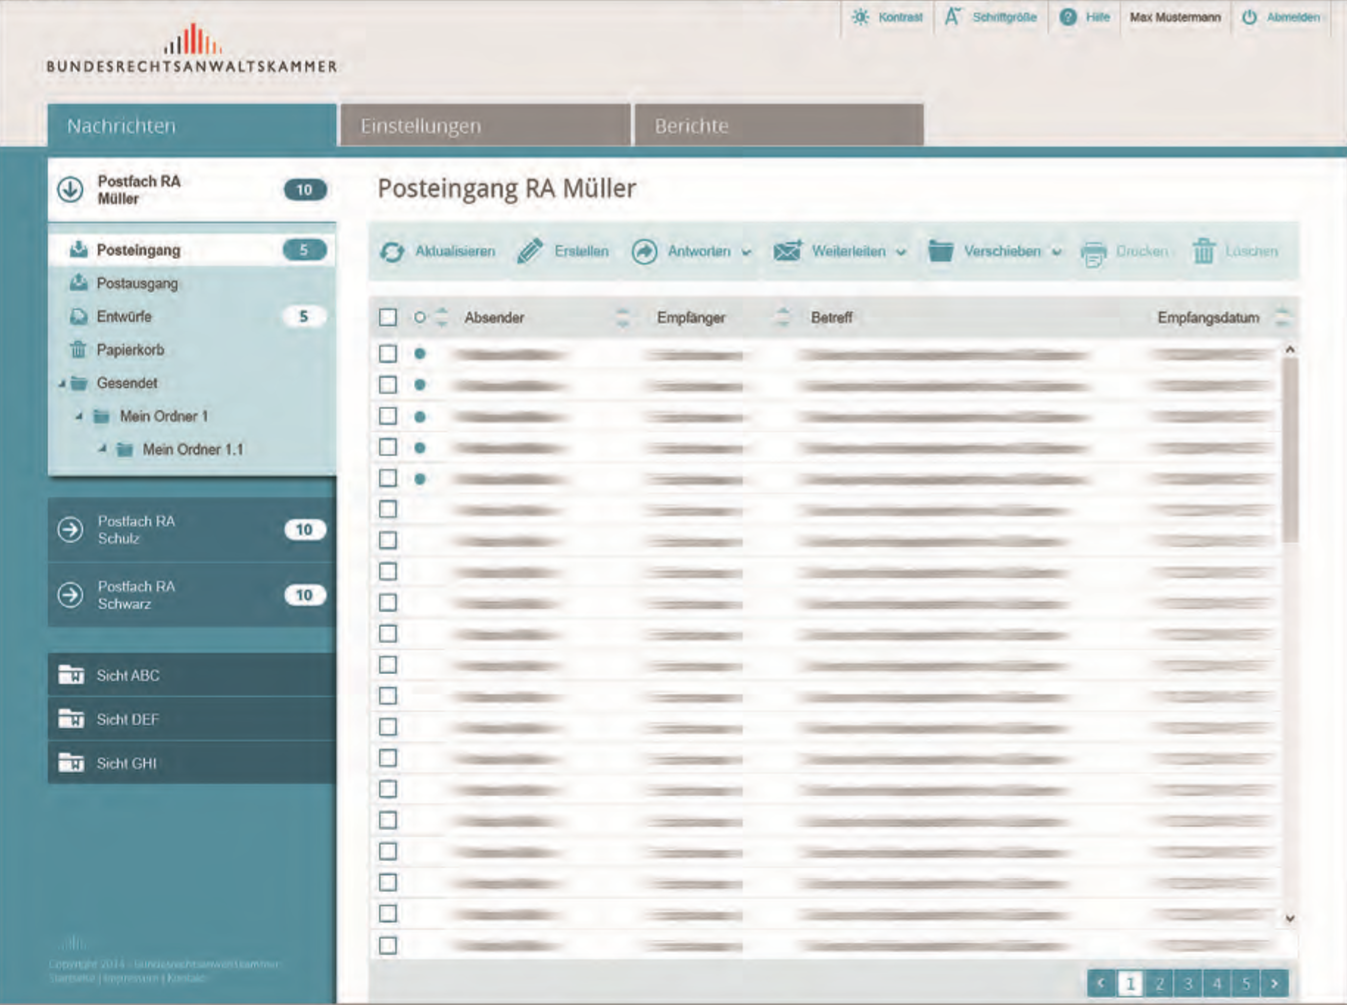
\includegraphics[width=\textwidth]{beA-ui1.png}
	\label{bea:gui:overview}
\end{center}

In Abbildung \ref{bea:gui:overview} ist die vorläufige Oberfläche des beA zu sehen. Man findet die typischen Ordner Posteingang und -ausgang, Entwürfe, Papierkorb und Gesendet vor, auf die der angemeldete Nutzer Zugriff hat. Beim beA kann der jeweilige Rechtsanwalt nur sein eigenes Postfach einsehen. Allerdings kann man Mitarbeitern bestimmte Rechte zuweisen, damit diese beispielsweise den Posteingang sehen und lesen können. Dadurch ist es auch möglich Urlaubsvertretungen festzulegen. Insgesamt wird es mehr als 30 Rechte geben, die man als Postfachinhaber an andere vergeben kann. Darunter fallen Lese-Rechte für bestimmte Ordner, das Recht Nachrichten zu versenden oder sogar das Recht, Rechte an andere vergeben zu dürfen. Durch dieses Rechte-System soll das geforderte jedoch nicht umgesetzte Kanzlei-Postfach simuliert werden. \\
''[...] Einen Wermutstropfen gibt es allerdings: Ein separates Kanzlei- oder Sozietätspostfach wird es nicht geben. Der Gesetzgeber wollte eine eindeutige Adressierbarkeit des einzelnen Rechtsanwaltes gewährleisten und hat daher in der BRAO festgelegt, dass nur Rechtsanwälte ein Anwaltspostfach erhalten. Um hier aber für anwaltliche Organisationseinheiten dennoch ein komfortables Arbeiten zu ermöglichen, gibt es so genannte Sichten (siehe Abbildung \ref{bea:gui:sichten}), die frei definierbar sind. Beispielsweise ist postfachübergreifend die Ansicht aller ungelesenen Nachrichten einstellbar, so dass eine Mitarbeiterin auf einen Blick alle neuen Nachrichten aus allen Postfächern, für die sie zugriffsberechtigt ist, sehen kann. So entsteht faktisch ein ''virtuelles Kanzleieingangspostfach''. Niemand muss sich durch alle Postfächer einzeln durchklicken. [...]''\cite{bea:bea:brak3-2015} \\
Allerdings können nur Rechte für Personen vergeben werden, die auch im Verzeichnis des beAs zu finden sind, demgemäß zugelassene Rechtsanwälte. In der Realität wird die Post eines Anwalts in Kanzleien meist nicht verwaltet, es gibt Sekretäre oder Sekretärinnen, die sich darum kümmern. Meist handelt es hierbei nicht um zugelassene Rechtsanwälte, weshalb sie auch keinen Zugriff auf das besondere elektronische Anwaltspost haben und damit auch keine Rechte zugewiesen bekommen können. Dies wird sich in der Praxis durch die hohen Sicherheitsvorkehrungen gewiss als hinderlich erweisen.

\subsection{Wie werden Nachrichten versendet?}
Das Versenden einer Nachricht gleicht dem einer E-Mail. Aufgrund der Ende-zu-Ende-Verschlüsselung ist der Nachrichtenbetreff nicht einsehbar, da er auch verschlüsselt wird. Lediglich die Identität des Absenders und das Datum kann man im Klartext lesen. Wurde die Nachricht seitens des Empfängers einmal geöffnet und damit entschlüsselt, ist der Betreff lesbar. Wird sie hiernach geschlossen, wird der Nachrichten-Inhalt inklusive aller Anhänge abermals verschlüsselt, der Betreff bleibt fortan in der Nachrichtenübersicht lesbar. Die Ursache hierfür ist der zweistufige Sicherheitscontainer des Sicherheitsprotokolls OSCI, welches für das Verschlüsseln der Nachrichten verantwortlich ist. Hier werden Inhalts- und Nutzungsdaten streng voneinander getrennt und können dadurch kryptographisch unterschiedlich behandelt werden. Dies ist vor allem für die Datenvermittlung notwendig.\cite{bea:osci} Weitere Details über das Sicherheitsprotokoll OSCI sind im Kapitel \ref{sec:bea:sicherheit:osci} zu finden. \\
Nachrichten liegen niemals unverschlüsselt im beA-System vor. Eingegangene Nachrichten können wie bei herkömmlichen E-Mail-Clients nach Belieben sortiert werden, um so schnellsten Zugriff und Übersicht zu erreichen.
Eine weitere wichtige Neuerung ist das elektronische Empfangsbekenntnis. Ab Anfang 2018 wird es dieses als maschinenlesbaren Datensatz geben, der automatisch ausgestellt, zurückgeschickt und anschließend eingelesen werden kann. Bis dahin kann ein Empfangsbekenntnis auf dem normalen Weg - sprich per Post oder Fax, oder qualifiziert elektronisch signiert als Anhang einer beA-Nachricht verschickt werden. 

\begin{figure}[ht]
	\subfigure[Sichten im Postfach]{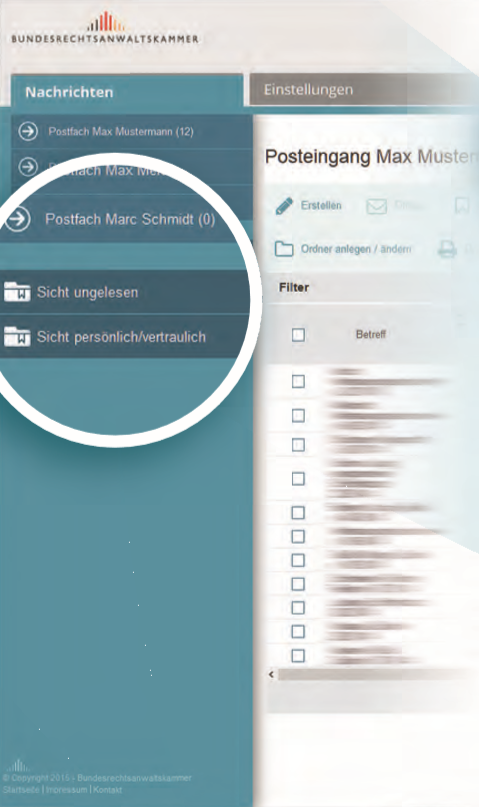
\includegraphics[width=0.49\textwidth]{beA-ui2.png}}
	\subfigure[Postfächer]{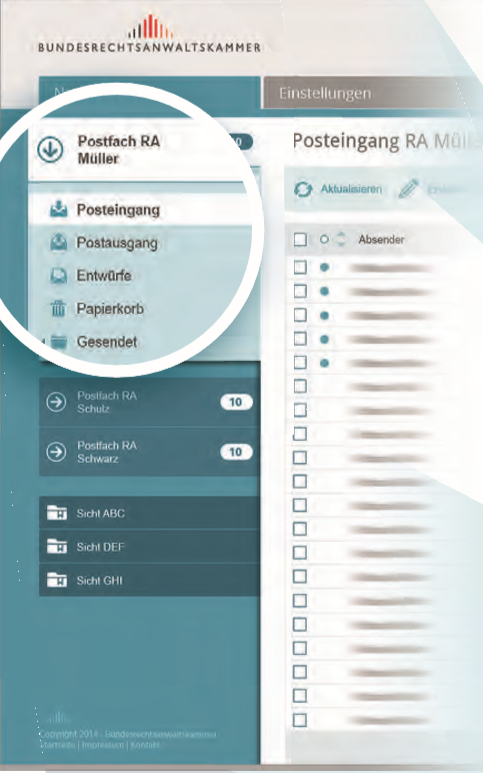
\includegraphics[width=0.49\textwidth]{beA-ui3.png}}
	\caption{Die Navigation innerhalb des Postfachs}
	\label{bea:gui:sichten}
\end{figure}


\subsection{Nachrichten versenden und weiterbearbeiten}
Der Versand der beA-Nachrichten gestaltet sich recht einfach. Es gibt ein Adressverzeichnis, in dem alle Gerichte, Rechtsanwälte, Kammern und sonstige Empfänger, die über das beA erreicht werden können, aufgelistet sind. Dabei ist zu beachten, dass noch nicht alle Gerichte das beA ab dem 01.01.2016 unterstützen werden. \\
Die Absenderzeile wird vom System automatisch ausgefüllt. Für die maschinelle Verarbeitung und Struktur ist es möglich das eigene und das gerichtliche Aktenzeichen und das der Gegenseite anzugeben. Diese Daten werden beispielsweise als Nutzungsdaten behandelt und dadurch vom OSCI-Standard anders verschlüsselt, als der Nachrichteninhalt. Folglich sind sie - wie bereits im vorigen Kapitel erwähnt, nach dem ersten Entschlüsseln sichtbar. Typischerweise können auch Anhänge zur Nachricht hinzugefügt werden. ''[...] In der Regel wird es sich dabei um Schriftsätze und deren Anlagen handeln. Bezüglich der Nachrichtengröße und der Anzahl der Anhänge orientiert sich das beA an den Vorgaben der Justiz, die voraussichtlich der Hauptadressat von beA-Nachrichten sein wird. Da eine Nachricht gleichzeitig an mehrere Empfänger adressiert werden kann, z.B. an ein Gericht und einen Anwalt, kann für die Kommunikation zwischen Rechtsanwälten nichts anderes gelten. Nach den Vorgaben des Justizstandards dürfen Nachrichten derzeit nicht größer als 30MB sein und nicht mehr als 100 Anhänge umfassen. Die Erweiterung auf 150 MB und 500 Anhänge ist bereits beschlossen. Die verwendbaren Dateiformate richten sich nach den Rechtsverordnungen der Länder, das beA macht hier keine Vorgaben. Einschränkungen wird es nur bei Dateiendungen geben, die eindeutig auf eine Schadsoftware hinweisen. [...]'' \cite{bea:bea:brak3-2015} \\
Am 01.01.2018 tritt der neue § 130a ZPO \cite{bea:bea:zpo130} in Kraft. Dann können Nachrichten über das \textit{besondere elektronische Anwaltspostfach} auch ohne qualifizierte elektronische Signatur (kurz qeS) verschickt werden. Hier gilt zu beachten, dass für die Übertragung der Nachricht zu einem Gericht ein sicherer Übermittlungsweg gewählt wird. Das beA stellt einen solchen Weg dar. Allerdings muss die Nachricht vom Postfachinhaber selbst abgeschickt worden sein. Hat ein Mitarbeiter das Recht erlangt, Nachrichten in einem anderen Postfach zu versenden, muss diese Nachricht trotz allem qualifiziert elektronisch signiert werden, um zu jeder Zeit den Absender eindeutig identifizieren zu können. \\
Bis zu diesem Zeitpunkt werden Nachrichten ohne qeS gar nicht erst verschickt werden können. Dafür soll bei der Umsetzung des beA Sorge getragen werden. \\
\\
Eingegangene Nachrichten können - wie bei herkömmlichen E-Mail-Clients, beantwortet oder zu einem anderen beA-Postfach weitergeleitet werden. Zudem kann man Nachrichten ausdrucken oder exportieren. Das beA ist, aufgrund der benötigten Kapazität und damit verbundenen Kosten, kein Nachrichtenarchiv. ''[...] Nachrichten sollten daher nicht im beA belassen werden, sondern in regelmäßigen Abständen in das eigene Dateiablagesystem exportiert oder ausgedruckt und gelöscht werden. Die BRAK wird voraussichtlich innerhalb des ersten Jahres nach Inbetriebnahme des beA-Systems Fristen festlegen, nach deren Ablauf der Postfachinhaber darüber informiert wird, dass Nachrichten automatisch in den Papierkorb verschoben und später dann gelöscht werden. [...]'' \cite{bea:bea:brak3-2015}

\subsection{Sicherheitstechnische Mittel}
Sicherheit - heißt Vertraulichkeit, Integrität, Authentizität, Verfügbarkeit und Verbindlichkeit, hat beim ERV und damit beim beA oberste Priorität. Findet ein Datenaustausch zwischen zwei Parteien statt, so soll gewährleistet werden, dass beide Parteien ihren Gegenüber eindeutig identifizieren können, kein Dritter den Datenaustausch manipulieren oder im Klartext lesen und dass der Austausch der Daten eindeutig den beiden Parteien zugeordnet werden kann. Dazu werden verschiedene sicherheitstechnische Mittel verwendet, die im Folgenden erläutert werden.

\subsubsection{Ende-zu-Ende-Verschlüsselung}\hspace*{\fill} \\
Vertraulichkeit und Integrität werden durch die sogenannte Ende-zu-Ende-Verschlüsselung einer beA-Nachricht gewährleistet. Bei dieser Verschlüsselung werden die Daten beim Sender verschlüsselt und erst beim Empfänger entschlüsselt. Dadurch können keine anderen Parteien während der Übertragung den Nachrichteninhalt im Klartext lesen. Um sich gegen sogenannte Man-In-The-Middle-Attacken zu schützen, generieren beide am Datenaustausch teilnehmenden Parteien einen String-Identifier, der auf ihren öffentlichen Schlüsseln (mit denen die Nachrichten verschlüsselt werden) beruht. Dieser Identifier wird untereinander ausgetauscht. Stimmt der ausgetauschte mit dem eigenen überein, so kann davon ausgegangen werden, dass niemand die Kommunikation belauscht. Jedoch bleiben bei einer solchen Ende-zu-Ende-Verschlüsselung dennoch Risiken: die beiden Endpunkte. Wurde der eigene Computer infiziert, so können Angreifer den privaten Schlüssel (Signaturschlüssel) stehlen, der zur Entschlüsselung von übersandten Nachrichten benutzt wird. \\
Im Gegensatz zum Verschlüsselungssystem zur De-Mail können damit weder Administratoren noch die BRAK selbst Nachrichten auf dem Server mitlesen.

\subsubsection{Sicherheitskarte}\hspace*{\fill} \\
Die Sicherheitskarte stellt ein physisches Medium dar, auf dem Schlüssel zum Verschlüsseln oder elektronisch Signieren von Nachrichten aufbewahrt werden. Damit lassen sich zum Beispiel auch Login-Verfahren sichern, in dem die an den Server übermittelten Daten sowohl signiert als auch verschlüsselt werden können. Dies hat den Vorteil, dass Angreifer auch die Sicherheitskarte stehlen müssten. Man fügt so dem klassischen Authentifizierungsverfahren mittels Benutzerkennung und Passwort eine zweite Sicherheitskomponente hinzu. Um die Karte benutzen zu können, braucht man ein Kartenlesegerät und eine spezielle Kryptographie-Software auf dem Computer. Laut Gesetz zum beA muss dieses Kartenlesegerät ein Gerät mit eigener Eingabetastatur besitzen. Andernfalls könnten sogenannte KeyLogger, Programme, die die Tastaturanschläge aufzeichnen, die PIN für die Karte herausfinden und an Dritte übermitteln. Die Kryptographie-Software wird benutzt, um Nachrichten oder Dokumente zu verschlüsseln und entschlüsseln oder elektronisch zu signieren beziehungsweise eine elektronische Signatur zu überprüfen. Hierzu wird je ein paar von Schlüsseln benutzt, die verschieden sind, sich jedoch eindeutig einander zuordnen lassen. Dabei handelt es sich um einen privaten Schlüssel - den Signaturschlüssel, und einen öffentlichen Schlüssel - den Signaturprüfschlüssel. Der private Schlüssel bleibt geheim, während der öffentliche Schlüssel jedem zugänglich ist. Der Signaturprüfschlüssel ist eindeutig dem Besitzer zugeordnet. Eine Nachricht oder Dokument, welches vom privaten Schlüssel signiert wurde, kann nur mit dem öffentlichen Schlüssel überprüft werden. Dadurch kann der Absender einer signierten Nachricht immer eindeutig festgestellt werden. Wird der Inhalt während der Übertragung verändert, ändert sich damit auch die Prüfsumme der Nachricht und der Signaturprüfschlüssel schlägt fehl. Damit gewährleistet dieses Verfahren Authentizität und Integrität.

\subsubsection{S.A.F.E.}\hspace*{\fill} \\
Secure Access to Federated eJustice/E-Government (kurz S.A.F.E.) ist ein bundesweiter Dienst für die deutsche Verwaltung, der Anwendungen sichere elektronische Identitäten (eIDs) für Personen und Organisationen zur Verfügung stellt. Dadurch können diese Personen beziehungsweise Organisationen durch ihre eID eindeutig identifiziert werden. \cite{bea:safe} Diese eID gilt für alle Dienste, sogenannte Trust-Domains, die von S.A.F.E. anerkannt werden. Registriert man sich bei einem dieser Trust-Domains erhält man eine eID. Damit ist man auch bei allen anderen Trust-Domains mit dieser eID registriert. Das Netzwerk für die Kommunikation zu und zwischen Trust-Domains wird über etablierte Standards abgewickelt, wie zum Beispiel das OSCI-Protokoll. Das beA stellt eine solche Trust-Domain dar, jeder Rechtsanwalt hat seine eigene eID.

\subsubsection{OSCI}\hspace*{\fill} \\
\label{sec:bea:sicherheit:osci}
''OSCI-Transport (Online Services Computer Interface Transport) ist ein Protokollstandard zur vertraulichen und sicheren Übermittlung von Nachrichten in einer auf das deutsche Signaturgesetz abgestimmten Sicherheitsumgebung. OSCI steht dabei für mehrere Protokoll, deren gemeinsames Merkmal die besondere Eignung für das E-Government ist:
\begin{itemize}
	\item OSCI-Transport für die sichere, vertrauliche und rechtsverbindliche Übertragung digitaler Daten über das Internet sowie
	\item eine Reihe verschiedener Protokolle (OSCI-XÖV-Standards) für den Austausch fachlicher Inhaltsdaten auf XML-Basis zwischen Kunden und Behörden bzw. Behörden untereinander.'' \cite{bea:osci}
\end{itemize}

OSCI-Transport-Nachrichten haben einen zweistufigen Sicherheitscontainer. Das bedeutet, dass Inhalts- und Nutzungsdaten voneinander getrennt und kryptografisch unterschiedlich zu behandelt werden können. Dabei werden beide Datensätze getrennt verschlüsselt. Danach werden sie in einen zweiten Sicherheitscontainer eingelegt, wobei dieser abermals verschlüsselt wird. Aufgrund dieses Prinzips spricht man in der Praxis auch oft vom ''Prinzip des Doppelten Umschlages''. Nachrichten werden immer Ende-zu-Ende-verschlüsselt. \\
Der Vorteil der Trennung von Inhalts- und Nutzungsdaten ist, dass der Intermediär nur die Nutzungsdaten sehen kann und damit auch zum Beispiel das beigefügte Aktenzeichen, wodurch dieser die Nachricht an die richtige Institution weiterreichen kann, ohne den tatsächlichen Inhalt lesen zu müssen. Die Inhaltsdaten können dadurch auch vom Nutzer eigenständig elektronisch signiert oder verschlüsselt werden, ohne, dass das System beeinträchtigt wird. \\
Jeder Sicherheitscontainer (für Nutzdaten und Inhaltsdaten) erlaubt die elektronische Signatur und die Verschlüsselung des jeweiligen Inhalts. Dadurch sind Vertraulichkeit, Integrität und Authentizität der Nachrichten gewährleistet. \cite{bea:osci}

\subsubsection{Erstanmeldung}\hspace*{\fill} \\
Bevor ein Rechtsanwalt das besondere elektronische Postfach benutzen kann, muss sich dieser dort zuerst anmelden. Diese Erstanmeldung verknüpft das Postfach mit der Identität des Rechtsanwalts, weshalb dieser Vorgang besonders sicherheitssensibel ist. Dazu benötigt er eine besondere beA-Karte, die die Postfachnummer als auch die eID enthält. Nach Inbesitznahme des Postfachs kann die beA-Karte auch zur täglichen Anmeldung genutzt werden.

\subsection{Das beA in der Praxis}
In den letzten Kapiteln haben wir das besondere elektronische Anwaltspostfach sowohl aus rechtlicher als auch aus technischer Sicht durchleuchtet und vorgestellt. In diesem Kapitel geht es um die Anwendung des Systems in der Praxis, wie gut sich das beA in den Alltag integriert und welche Vor- beziehungsweise Nachteile es mit sich bringt. \\
Durch den elektronischen Rechtsverkehr muss eine stete Erreichbarkeit der Dienste gewährleistet werden, damit auch bestimmte Fristen eingehalten werden können. Jedoch werden, wie bei jedem anderen Dienst auch, Wartungsarbeiten durchgeführt werden müssen. Zu dieser Zeit wird das System nicht verfügbar sein.
Ist die Übertragung eines elektronischen Dokuments aus technischen Gründen nicht möglich, bleibt die Übermittlung dennoch zulässig. Das Dokument muss folglich nachgereicht und es muss glaubhaft gemacht werden, dass eine Übermittlung nicht möglich gewesen ist (siehe § 130d S. 2 ZPO n. F.\cite{bea:bea:zpo130}). \\
Eine ähnliche Situation bietet sich, falls ein elektronisches Dokument vom Gericht nicht verarbeitet werden kann. Nach der Übertragung wird dies dem Absender mitgeteilt und der Zeitpunkt dieser Einreichung gilt, solange der Absender glaubhaft machen kann, dass das nachgereichte Dokument mit dem zuvor übermittelten übereinstimmt (siehe § 130a Abs. 6 ZPO n.F). \\
\\
Zudem entstehen gegebenenfalls weitere Kosten, um das beA nutzen zu können. Laut der Bundesrechtsanwaltkammer bedarf es folgender Voraussetzungen:
\begin{itemize}
	\item eine leistungsfähige Internetverbindung (mind. 2mbit/s),
	\item ein Computer mit mind. 512 MB Arbeitsspeicher und AMD- oder Intel-Prozessor,
	\item das aktuelle Betriebssystem: Windows, MacOS oder Linux,
	\item (beA-)Signaturkarte und Kartenlesegerät \textbf{mit Tastatur} und
	\item Drucker und Scanner. \cite{bea:bea:brak}
\end{itemize}
Da eine Datenrate von 2 Mbit/Sekunde leider noch nicht überall in Deutschland verfügbar ist, wurde der rechtliche Rahmen im ERV-Gesetz so gestaltet, dass bei nachgewiesener Unmöglichkeit einer elektronischen Übersendung zum Gericht auch ein konventioneller Versand möglich sein wird. Dennoch ist dieser Zustand unbefriedigend: Die BRAK wird sich deshalb auf allen politischen Kanälen für einen zügigen Ausbau des Breitbandnetzes einsetzen. Immerhin haben die Regierungsfraktionen in ihrer Koalitionsvereinbarung von 2013 versprochen, dass es bis 2018 in Deutschland eine flächendeckende Grundversorgung mit mindestens 50 Mbit/Sekunde geben soll. \\
\\
Um das beA effektiv in der Kanzlei einzusetzen, ist in der Regel ein Drucker, ein Scanner oder eine Kombination aus beiden erforderlich. Der Scanner sollte auf verschiedene Auflösungen einstellbar sein, so dass die Pixeldichte je nach Dokumententyp – Textdatei oder Bilddatei – individuell einstellbar ist. Eine geringere Auflösung bedeutet eine geringere Dateigröße und damit einen einfacheren Versand der Nachrichtenanhänge. \\
Sicher bedeuten diese Anschaffungen zunächst einmal einen gewissen finanziellen Aufwand für jede Kanzlei. Dem gegenüber stehen jedoch deutliche Ersparnisse bei den Papier- und Portokosten und vor allem auch langfristig Vereinfachungen in den alltäglichen Arbeitsabläufen. Dabei fügt sich das beA selbstverständlich umso besser in den Arbeitsalltag ein, je stärker die Kanzlei an sich digitalisiert ist. Auch wenn die Nutzung des beA eine elektronische Aktenführung nicht voraussetzt, bietet die Einführung doch eine gute Gelegenheit auch insgesamt über eine Digitalisierung der Kanzlei nachzudenken

\subsubsection{Anwälte}\hspace*{\fill} \\
Anwälte erhalten mit dem beA keine herkömmliche E-Mail-Adresse, sondern ihre Adressdaten liegen in einer Datenbank. Nachrichten werden direkt an den jeweiligen Rechtsanwalt oder das jeweilige Gericht geschickt.
Der Begriff des Anwaltspostfachs ist dabei irritierend. Das Postfach ist nicht öffentlich, sondern nur die Adresse innerhalb des Systems. Der Anwalt kann zudem keine Nachrichten an Personen schicken, die selbst kein Anwaltspostfach besitzen. Eine Kommunikation mit dem Mandanten ist über das beA aus diesem Grund nicht möglich. Dies führt dazu, dass Rechtsanwälte zwangsläufig mindestens zwei Kommunikationsmittel parallel benutzen müssen. \\
Die Kosten für die Einrichtung der besonderen elektronischen Anwaltspostfächer werden im Ergebnis von der Anwaltschaft zu tragen sein. ''[...] Für die Entwicklung des beA und die Bereitstellung der Betriebsumgebung erhebt die BRAK für die Jahre 2014 und 2015 zusammen einen Beitrag von 63 Euro pro Rechtsanwalt, der 2015 von den Rechtsanwaltskammern eingezogen wird. Die Kammern finanzieren diesen Beitrag unterschiedlich – teilweise durch eine Erhöhung der Mitgliedsbeiträge, teilweise durch eine Umlage und teilweise durch einen Rückgriff auf das Vermögen der jeweiligen Kammer. Die Beschlüsse dazu werden in den jeweiligen Kammerversammlungen durch die Mitglieder gefasst. Über die Beitragshöhe in den Folgejahren entscheiden die Rechtsanwaltskammern jeweils im Frühjahr. [...]'' \cite{bea:bea:brak}

\subsubsection{Kanzleien}\hspace*{\fill} \\
Die Einführung und Verpflichtung zur Nutzung haben auch Auswirkungen auf das Arbeiten in der Kanzlei. Das beA bietet eine Schnittstelle an, die die eventuell vorhandene Kanzleisoftware benutzen kann, um auf das Postfach zuzugreifen. Damit dies schlussendlich funktioniert, müssen die Kanzleien ihre internen Systeme und Strukturen auf die Benutzung des beA umstellen. Im Kapitel zur Umsetzung des beA haben wir bereits gesagt, dass es keine Kanzleipostfächer geben wird. Stattdessen können durch Rechtevergabe ''virtuelle Kanzleipostfächer'' erstellt werden. Das bedeutet, dass jede Kanzlei diese Postfächer zuerst erstellen muss, was zu erheblichem Mehraufwand führt.  
Das besondere elektronische Anwaltspostfach bringt andererseits auch Vorteile mit sich: Ein wesentlicher Vorteil ist der schnelle und sichere Datenaustausch mit Zustellungsnachweis. Durch die Eingangsbestätigung weiß der Anwalt, ob und wann die Nachricht bei Gericht angekommen ist. Außerdem können elektronische Strukturdaten, zum Beispiel Daten zu Aktenzeichen, mit dem Gericht ausgetauscht werden. Zudem können diese Strukturdaten automatisch von der Kanzleisoftware eingelesen und verarbeitet werden. Ein gutes Beispiel ist das automatische Auslesen von Fristen aus den Strukturdaten und Eintragen in den Kalender in der Kanzleisoftware. \\
Die elektronische Aktenführung bietet zudem eine enorme Flexibilität. Denn elektronische Akten sind zusätzlich von überall, wo ein Netzzugang vorhanden ist, abzurufen. Auch Akteneinsichten oder Verfahrensstandabfragen werden zukünftig elektronisch und dadurch dem Arbeitsplatz - sogar von zu Hause aus, möglich werden. Insofern ist ein permanenter und ortsunabhängiger Zugriff zu jeder Zeit möglich. Künftig wird man auch nicht mehr an die Öffnungszeiten der Gerichte gebunden sein, sondern hat – ohne Wartezeiten –  zeitlich unbegrenzten Zugriff auf die einzusehenden Dokumente.
Ein weiterer Vorteil ist die effizientere Arbeitsweise und Kostenreduzierung: Eine Kosteneinsparung ergibt sich bereits daraus, dass vor allem Portokosten für das Versenden von Schriftsätzen etc. oder für die Anforderung von Akten entfallen – ebenso die Kosten für Versandumschläge und das Ausdrucken oder Kopieren der Akten und Schriftsätze. Außerdem führt eine elektronische Archivierung der Akten dazu, Akten- und Papierberge zu vermeiden. Somit müssen auch keine zusätzlichen Räumlichkeiten mehr bereitgehalten werden, in denen die Akten aufbewahrt werden. Ebenso entfällt die umständliche Suche im Aktenkeller. \\
Eine elektronische Aktenführung ermöglicht zudem eine effektivere Mandatsbearbeitung, als es mit Papierakten möglich ist. Dadurch wird die Aktenbearbeitung effizienter und schneller, denn man kann Akten besser sortieren, findet sie schneller, kann Akten und im Inhalt der Akten suchen und kann diese zudem systematisch erfassen.

\subsection{Besonderes elektronisches Notarpostfach}
Notare nutzen ab dem 01.01.2016 das besondere Notarpostfach. Dessen Bereitstellung liegt im Verantwortungsbereich der Bundesnotarkammer. Dabei gleicht das Notarpostfach dem beA. Bisher haben Notare ein Postfach im EGVP besessen. \cite{bea:notarpostfach}
\section{EGVP}
Elektronisches Gerichts- und Verwaltungspostfach (kurz EGVP) ist ein Postfach für die Justiz, das von der öffentlichen Verwaltung, Bürgern, Unternehmen, Inkassogesellschaften, Rechtsanwälte, Notare oder Gerichtvollziehern über einen speziellen EGVP-Classic-Bürger-Client erreicht werden kann, um Dokumente elektronisch einzureichen. \\
Nachrichten, die über den EGVP-Client versendet werden, unterliegen dem OSCI-Sicherheitsstandard und sind damit auch, im Gegensatz zum Standardversand von Nachrichten bei der De-Mail, Ende-zu-Ende verschlüsselt. Mit der Einführung des besonderen elektronischen Anwalts- (kurz beA) beziehungsweise Notarpostfachs, wird der EGVP-Client obsolet, Ein Grund dafür ist sicherlich die geringe Akzeptanz des eher sperrigen und fehleranfälligen Clients. Ein anderer scheint gewiss die schlechte Integrität des EGVPs zu sein: erst in sechs Bundesländer kommt das EGVP zum Einsatz, allerdings auch bei diesen nicht an jedem Gericht. ''[...] Nur in Berlin, Brandenburg, Bremen, Hessen, Rheinland-Pfallz (Verwaltungs-, Sozial- und Finanzgerichtsbarkeit) und Sachsen können Schriftsätze und Klagen über das EGVP bei ordentlichen und besonderen Gerichtsbarkeiten eingereicht werden.
In manchen Bundesländern wird die Technik nur an ganz bestimmten Gerichten eingesetzt. In Hamburg ist es das Finanz-, in Schleswig-Holstein sind es die Arbeitsgerichte. Bis tatsächlich alle Gerichte in ganz Deutschland über die notwendige Technik für den neuen Standard verfügen werden, hat der Gesetzgeber eine Frist bis spätestens zum Jahr 2020 gelassen. Bis dahin jedoch ist das elektronische Anwaltspostfach, welches das EGVP ersetzen soll, ein Programm mit vielen Sendern – aber ein Großteil der wichtigsten Empfänger fehlt.'' \textcite{bea:egvp:landkarte}\footfullcite{bea:egvp:landkarte} \\
\\
Das EGVP findet eher wenig Verwendung, weshalb es vom besonderen elektronischen Anwalts- bzw. Notarpostfachs abgelöst wird. Dies ist im Gesetz zur Förderung des elektronischen Rechtsverkehrs festgelegt. Jedoch wurde von der Bund-Länder-Kommission für Informationstechnik (BLK) in der Justiz beschlossen, dass die Infrastrukturkomponenten für die Kommunikation, soll heißen die Postfächer und die Adressen im Verzeichnisdienst S.A.F.E, für Nutzer die weder Rechtsanwalt noch Notar sind, weiterhin unverändert zur Verfügung stehen werden. \textcite{bea:egvp}\footfullcite{bea:egvp} \\
Jedoch wird der EGVP-Bürger-Client, das bedeutet die Software zum Kommunizieren mit dem EGVP, am 01.01.2016 offiziell eingestellt, steht den Nutzern jedoch noch bis zum 30.09.2016 - allerdings ab dem 01.04.2016 ohne Support, zur Verfügung. Danach müssen Nutzer auf Software von Drittherstellern zurückgreifen. Die beschlossene Übergangsfrist, vom 01.01.2016 bis zum 01.04.2016, soll dabei den Rechtsanwälten und Notaren zu gute kommen. Sie stellt einen Zeitraum dar, in dem das besondere elektronische Anwalts- bzw. Notarpostfach und der EGVP-Bürger-Client parallel betrieben werden können, so dass der laufende Kanzleibetrieb nicht beeinträchtigt wird. \\
\\
Bürger, die einmalig oder selten Zugang zu Gerichten benötigen, können ab dem 01.10.2016 ein Online-Formular, das sogenannte Web-EGVP, benutzen. Mit diesem Formular können Nachrichten versandt werden, eine elektronische Rückantwort ist allerdings nicht möglich.
\section{De-Mail}
Der Staat reagierte auf die geringe Akzeptanz des EGVP mit dem De-Mail-Gesetz. Damit sollte die Grundlage für den verbindlichen, sicheren, vertraulichen und nachweisbaren Versand elektronischer Dokumente und Nachrichten gelegt werden.\textcite{bea:demail}\footfullcite{bea:demail} \\
Es gibt verschiedene De-Mail-Dienste, die dem Verbraucher zur Verfügung gestellt werden. Dazu gehören der Versand- und Postfachdienst, der De-Safe und der Dienst für zuverlässigen Identitätsnachweis, De-Ident. \\
Die De-Mail kann von Jedermann benutzt werden. Sie wird nicht vom Staat selbst bereitgestellt, stattdessen wurden zertifizierte Unternehmen beauftragt. Durch die Implementierung internationaler Standards können diese Unternehmen ihren Kunden eine sichere und rechtsverbindliche Kommunikation anbieten. Die De-Mail verfügt dabei über wichtige Eigenschaften, die eine herkömmliche E-Mail nicht hat:
\begin{itemize}
	\item Durch den De-Ident-Dienst können die Identitäten von Absender und Adressat eindeutig nachgewiesen und nicht gefälscht werden. 
	\item Nutzer des De-Mail-Versanddienstes können Nachrichten als Einschreiben verschicken. Dadurch erhalten sie eine qualifiziert signierte Bestätigung, wann die Nachricht abgeschickt und wann sie im Postfach des Empfänger angekommen ist.
	\item Der Versand von Nachrichten wird ausschließlich über verschlüsselte Kanäle getätigt. Im Postfach des Empfängers werden die Nachrichten nur verschlüsselt abgespeichert (De-Safe-Dienst). Dadurch sollen sie zu keiner Zeit von Dritten im Klartest gelesen oder gefälscht werden können.
\end{itemize}

Am 1. August 2013 ist E-Government-Gesetzes das Kraft getretenen. Unter bestimmten Voraussetzungen ist es nun auch möglich die in Verwaltungsakten erforderliche Schriftform durch den Versand einer De-Mail zu ersetzen. \\
Der De-Mail-Dienst sollte vor allem aufgrund der hohen Sicherheitsstandard für Bürgen und Behörden attraktiv gemacht werden. Allerdings weißt der Dienst erhöhte Mängel auf:
''Die hohe Relevanz und Vertraulichkeit der per De-Mail versendeten Dokumente erhöht die Attraktivität der De-Mail-Server als Angriffsziele. Dem entsprechend zu erwartenden Angriffsvolumen steht aufgrund der mangelnden Ende-zu-Ende-Verschlüsselung kein adäquates Sicherheitskonzept entgegen.'' \textcite{bea:demail:ccc}\footfullcite{bea:demail:ccc} Der De-Mail-Dienst verwendet authentisierte und verschlüsselte Kommunikationskanäle zwischen Nutzer und Anbieter, als auch zwischen Anbietern untereinander. Nachrichten werden erst auf Anbieter-Seite elektronisch signiert und verschlüsselt und danach zum Empfänger-Anbieter versandt. Dieser muss die Nachricht allerdings zuerst entschlüsseln, um die Integrität des Senders zu überprüfen. Danach wird die Nachricht abermals verschlüsselt und ins Empfänger-Postfach geschickt. Dadurch entstehen die hohen Sicherheitsmängel seitens der Anbieter. Aber auch die Tatsache, dass Nachrichten erst auf Anbieter-Seite vom Anbieter selbst signiert werden, erscheint unwirklich. Der Nutzer hat keinerlei Kontrolle und muss seinem Anbieter vertrauen, dass seine keine Fehler passieren oder seine elektronische Signatur nicht missbraucht wird. \\
Weiterhin muss lediglich beim Erstellen des De-Mail-Accounts ein Identitätsnachweis - meist in Form eines amtlichen Lichtbildausweises oder der eID-Funktion  des Personalausweises, erbracht werden. Anfänglich wurde danach nur Nutzerkennung und Passwort benötigt, um sich ins Postfach einzuloggen. Diesem Sicherheitsmangel sollte durch §4 (2) des De-Mail-Gesetzes durch die BSI durch das mTan-Verfahren zur verstärkten Sicherheit entgegengewirkt werden. Diese Neuregelung sieht einen zweiten Authentifizierungsweg zum Einloggen vor, wie zum Beispiel der Eingabe eines Authentifizierungscode der per SMS auf eine hinterlegte Mobilnummer entsandt wird. Aber auch das mTAN-Verfahren ist nicht sicher. Bislang wird dieses Konzept bei Banken verwendet und kann beispielsweise durch die Infektion des Telefons, Abhören von SMS-Inhalten oder durch Impersonierung, sprich Kopieren der SIM-Karte, angegriffen werden. \textcite{bea:demail:brokenbydesign}\footfullcite{bea:demail:brokenbydesign} \\
Ein weiterer Nachteil ist die fehlende Integration des Dienstes für den Versands an Postfächer des EGVP und der geringe Datenschutz\textcite{bea:demail}:
\begin{itemize}
	\item Laut §112 des Telekommunikationsgesetzes kann die Identität hinter einem De-Mail-Nutzerkonto von etwa 250 registrierten Behörden online abgerufen werden.
	\item Laut §113 des Telekommunikationsgesetzes sind die persönlichen Daten des Nutzers für eine Vielzahl von Sicherheitsbehörden und Geheimdienstes ohne richterliche Anordnung einsehbar.
\end{itemize}

Auf dem 30. Chaos Communication Congress stellte der Sicherheitsanalyst Linus Neumann seine Analyse ''Bullshit made in Germany'' des De-Mail-Dienstes vor. Er formulierte treffend: ''De-Mail [sei] absichtlich unsicher gebaut, um deutschen Diensten zu ermöglichen, deutsche Bürger auszuspähen.''\textcite{bea:demail:bullshit}\footfullcite{bea:demail:bullshit}
 


\section{Technische Aspekte}
Im vorherigen Kapitel haben sich als wichtige Anforderungen an den Rechtsverkehr und die elektronische Dokumente heraus kristallisiert:
\begin{itemize}
\item Authentizität und Integrität
\item Vertraulichkeit
\item Datenschutz persönlicher Daten
\end{itemize}
Um diese Anforderungen auf technische Ebene zu gewährleisten werden verschiedene Verfahren und Konzepte der Authentifizierung, Autorisierung und zur Erstellung von digitalen Signaturen eingesetzt. Im folgenden sollen gängige Verfahren vorgestellt werden um den notwendigen  technischen Hintergrund zu schaffen. 
\subsection*{Authentifizierung}
Es existieren viele verschiedene Authentifizierungsverfahren, welche sich in ihrer Komplexität unterscheiden. Die einfachsten Verfahren erwarten die Eingabe von Benutzername und Passwort. Allerdings gehören diese auch zu den unsichersten Verfahren. Damit eine Authentifizierung möglich ist, müssen eindeutige die Person identifizierende Eingaben vorliegen. Diese lassen sich in drei Kategorien unterscheiden.
\begin{itemize}
\item Wissen: Eingabe einer geheimen Information, beispielsweise ein PIN.
\item Gegenstand: Auslesen eines Gegenstandes,z.B. eine Karte oder ein USB-Token
\item Attribut: Ein Indentifikationsmerkmal der Person, beispielsweise das Augenmuster oder der Fingerabdruck eines Menschen.
\end{itemize}
\subsubsection{Multi-factor authentication}
Je nach Authentifizierungsverfahren reicht die Eingabe einer Information (Single Factor Authentication) oder es müssen mehrere Faktoren eingegeben werden (Multi Factor Authentication).
Dabei kann jeder Faktor die Person eindeutig identifizieren. Damit eine Authentifizierung erfolgreich ist müssen jedoch alle Eingaben korrekt sein. Bei der Multi Factor Authentication werden aus Sicherheitsgründen Faktoren aus unterschiedlichen Kategorien gewählt. Ein typisches Beispiel ist die Authentifizierung an einem Bankautomat. Dazu ist die Eingabe eines PINS, sowie einer Bankkarte notwendig. Nur wenn beide Faktoren vorliegen und zueinander passen ist die Authentifizierung erfolgreich. 
\subsubsection{Mutual authentication}
erlaubt dem Benutzer zu verifizieren, dass die Authentifizierung an dem gewünschten System erfolgreich war, sodass er nur nach einer erfolgreichen Authentifizierung seine sicherheitskritischen Daten ein gibt. \textit{Phishing Attacks} zielen darauf ab, Benutzern eine Authentifizierung  vorzutäuschen, sodass sie danach z.B. ihr Passwort eingeben, obwohl sie nicht mit dem gewünschten System verbunden sind.


\subsubsection{Shared Secrets (Passwords)}
\textit{Shared Secrets} wie Passwörter oder PINS sind die meist genutzten Schlüssel um Sicherheit zu gewährleisten und Zugriff auf Online Portale erlauben. Ein Problem dabei ist jedoch, dass die Erfahrung gezeigt hat, dass Menschen dazu neigen schlechte Passwörter zu wählen, sie leicht offen legen, oder ihre Passwörter vergessen. Dies macht es einfach für einen Spezialisten das Passwort zu stehlen. 
\subsubsection{One time passwords (otp)}
Ein \textit{One time password} ist ein Passwort, welches sich für jede Verwendung ändert. Es werden zwei grundlegende Möglichkeiten unterschieden, wie ein \textit{One time password} funktioniert:
\begin{itemize}
\item Es wird eine Liste von Tans generiert, die zwischen dem Benutzer und System geteilt wird. Bei jeder Verwendung wird der Benutzer nach einer der Tans gefragt.
\item Bei jeder Passworteingabe wird das Passwort vom Benutzer neu generiert und vom System verifiziert. Dabei kann das Passwort z.B. eine Funktion von der aktuellen Zeit sein, welches der Benutzer und das System teilen.
\end{itemize}
\subsubsection{SSL/TLS Protokoll}
SSL/TLS sind Protokolle, die für den sicheren Austausch von Informationen zwischen Client und Server genutzt werden. Im folgenden wird kurz der Vorgang eines \textit{SSL Handshake} unter Nutzung des \textit{RSA exchange} Algorithmus beschrieben:
\begin{enumerate}
\item \textit{Client Hello:} Der Client sendet für die SSL Kommunikation notwendige Informationen wie z.B. die SSL Version.
\item \textit{Server Hello:} Der Server antwortet mit für den Client relevanten Informationen, u.a. mit dem SSl Zertifikat des Servers (Public Key).
\item  Der Client überprüft das Zertifikat auf Korrektheit.  Ist dies gegeben, erzeugt der Client den Schlüssel für die spätere Kommunikation und verschlüsselt ihn mit dem \textit{Public Key} des Servers.
\item Der Server entschlüsselt den Schlüssel mit dem Private Key.
\item Für die Session wird der Session Schlüssel zur Verschlüsselung der Kommunikation genutzt.
\end{enumerate}	
\subsection*{Autorisierung/Zugriffskontrolle}

Der Sinn und Zweck von Zugriffskontrolle ist die erlaubten Operationen auf einen Datensatz einzuschränken. In der Informatik beschränken Zugangsberechtigungen sowohl die erlaubten Operationen eines Nutzers als auch die eines Programms. In diesem Sinne soll Zugriffskontrolle alle Operationen, welche die Sicherheit einschränken, verhindern. Im folgenden werden verschiedene Grundsätze der Zugriffskontrolle beschrieben.

\subsubsection{Voraussetzung}
Damit Zugriffskontrolle möglich ist, muss das System den Benutzer erkennen. Dies bedeutet, dass sich der Benutzer in einem ersten Schritt in dem System anmelden muss(vgl. Authentifizierung). Vor jeder Anfrage muss erneut überprüft werden, ob der Benutzer die nötigen Berechtigungen besitzt.
\subsubsection{Zugriffssteuerungsmatrix}
Die Zugriffssteuerungsmatrix ist ein abstraktes Sicherheitskonzept, welches jedem Benutzer zu jedem Objekt gewisse Rechte zuweist. Das bedeutet insbesondere, dass für jedes Objekt unterschiedliche Berechtigungen gelten können. Es wurde 1971 von Butler W. Lampson eingeführt(Quelle).
\subsubsection{Rollenbasierte Zugriffskontrolle}
Role Based Access Control (RBAC; deutsch: Rollenbasierte Zugriffskontrolle) ist in Mehrbenutzersystemen oder Rechnernetzen ein Verfahren zur Zugriffssteuerung und -kontrolle auf Dateien oder Dienste. Das RBAC-Modell wurde 1992 von D.F. Ferraiolo und D.R. Kuhn beschrieben[1] und 2004 als ANSI-Norm 359-2004 verabschiedet.
\\\\
Die alternative Methode, einem realen Benutzer (User) direkt Rechte und Zugriffe auf verschiedene Systeme zu geben, stellte sich durch die steigende Zahl von Benutzern als unübersichtlich und daher fehlerträchtig dar. Das auf Benutzerrollen basierende Konzept soll nun die Rechte anhand von Arbeitsprozessen abstrahieren.
\\\\
Bei der rollenbasierten Zugriffskontrolle werden den Benutzern des Computers oder Netzwerks Rollen zugeordnet. Benutzer können dabei mehrere Benutzerrollen besitzen. An eine Rolle sind beispielsweise 1 bis n Gruppenzugehörigkeiten gebunden. Je nach Rollenzuordnung des Benutzers (und den damit verbundenen Gruppenzugehörigkeiten) erteilt oder sperrt das System dann das Zugriffsrecht auf Betriebsmittel. Häufig werden vor allem Lesen, Schreiben und Ausführen von Dateien mittels RBAC kontrolliert; das Verfahren ist jedoch nicht darauf beschränkt.

\subsubsection{Militär Sicherheitsbestimmung}
Das Prinzip der Militär Sicherheitsbestimmung ist es Informationen basierend auf ihrer Sicherheitsstufe zu klassifizieren. Es wird unterschieden zwischen
\begin{itemize}
\item unclassified
\item restricted
\item confidential
\item secret 
\item topsecret
\end{itemize} 
Jeder Information ist ein Tupel aus Rang und Kompartiment zugeordnet. Dabei bestimmt das Kompartment zu welchen Projekten die Information gehört. 
Eine Person kann auf Informationen bis zu einer gewissen Sicherheitsstufe zugreifen. Die Zugangsberechtigung einer Person wird ebenfalls als Tupel aus Rang und Kompartiment dargestellt.   
\subsubsection{Bell-LaPdula Modell}
Das \textit{Bell-LaPdula Modell} ähnelt dem \textit{Military security policy}. Zusätzlich werden unterschiedliche Schreib- und Leserechte definiert. Insbesondere kann kein Datensatz höherer Sicherheitsstufe gelesen und kein Datensatz mit niedriger Sicherheitsstufe geschrieben/bearbeitet werden.
\subsubsection{Conditional Policies}
\textit{Conditional Policies} bedeutet, dass Sicherheitskriterien zusätzlich zu den bereits genannten Punkten auch abhängig von dem aktuellen Kontext des Benutzers sein können. Beispielsweise kann der Zugang zu speziellen Daten, nur von einem bestimmten Ort und auch nur für einen gewissen Zeitraum freigeschaltet werden.
\subsubsection{Biba Modell}
Das \textit{Biba Model} dient der Wahrung der Integrität. Es beinhaltet das Daten einer niedrigeren Sicherheitsstufe wie der Benutzer nicht gelesen und Daten einer höheren Sicherheitsstufe nicht geschrieben werden dürfen. Es ist damit eine Umkehrung des \textit{Bell-LaPdula Modells}.
\subsubsection{Separation of duty}
Das Prinzip \textit{Separation of duty} besagt, dass für eine wichtige Aufgabe immer mehr als eine Person verantwortlich sind. Dies beinhaltet das wichtige Entscheidungen nur unter Zustimmung aller Verantwortlichen getroffen werden dürfen. Dadurch sollen sowohl Fehler als auch Machtmissbrauch verhindert werden
\subsubsection{Chinese Wall Policy}
Nach dem \textit{Chinese Wall Policy} darf ein Benutzer nur auf Daten zugreifen, die nicht im Konflikt mit anderen Daten stehen, welche dem Benutzer zur Verfügung stehen. Dadurch soll ein Interessenkonflikt des Benutzers vermieden werden. 
\subsubsection{Principle of Least Privilege}
Das \textit{Principle of Least Privilege} besagt, dass Personen nur auf diejenigen Daten zugreifen dürfen, die für ihre Arbeit zwingend erforderlich sind.
\subsection*{Digitale Signaturen}
Eine digitale Signatur, auch digitales Signaturverfahren, ist ein asymmetrisches Kryptosystem, bei dem ein Sender mit Hilfe eines geheimen Signaturschlüssels (dem Private Key) zu einer digitalen Nachricht (d. h. zu beliebigen Daten) einen Wert berechnet, der ebenfalls digitale Signatur genannt wird. Dieser Wert ermöglicht es jedem, mit Hilfe des öffentlichen Verifikationsschlüssels (dem Public Key) die nichtabstreitbare Urheberschaft und Integrität der Nachricht zu prüfen. Um eine mit einem Signaturschlüssel erstellte Signatur einer Person zuordnen zu können, muss der zugehörige Verifikationsschlüssel dieser Person zweifelsfrei zugeordnet sein.

Mit digitalen Signaturen lassen sich sichere elektronische Signaturen (fortgeschrittene elektronische Signaturen gem. § 2 Nr. 2 SigG bzw. qualifizierte elektronische Signaturen gem. § 2 Nr. 3 SigG) erzeugen. Die Begriffe digitale Signatur und elektronische Signatur sind jedoch nicht inhaltsgleich: Erstens müssen (zumindest fortgeschrittene) elektronische Signaturen nicht zwangsläufig auf digitalen Signaturen basieren; zweitens ist digitale Signatur ein mathematischer bzw. technischer Begriff, während elektronische Signatur ein juristischer Begriff ist.
\subsubsection{Gesetzliche Normen}
Die Bundesnetzagentur veröffentlicht jedes Jahr eine Liste mit Mindestanforderungen für kryptographische Algorithmen für die Erzeugung qualifizierter elektronischer Signaturen.[2] In der „Bekanntmachung zur elektronischen Signatur nach dem Signaturgesetz und der Signaturverordnung“ vom 18. Januar 2012 werden als geeignete digitale Signaturverfahren RSA , DSA und DSA-Varianten die auf elliptischen Kurven basierend (z. B. EC-DSA, EC-KDSA, EC-GDSA) empfohlen. Zu jedem dieser Verfahren werden die Mindestlängen für die Schlüssel sowie weitere Anforderungen an die Parameter und die Hashfunktion angegeben. [3]
\subsubsection{RSA}
In der modernen Kryptologie hat sich die RSA – Verschlüsslung als eine der
sichersten Methoden durchgesetzt. Sie wird heute in wichtigen Bereichen wie  im
Bankenwesen (z.B. bei der Verschlüsslung von Geheimzahlen) eingesetzt.
\\\\
Leonard Euler entdeckte eine mathematische Regel, die für die RSA –
Verschlüsselung grundlegend ist. Wählt man zwei positive Primzahlen $p$ und $q$ mit $p \neq q$, dann gilt:
\begin{equation}
	\begin{split}
		m^{s(p-1)(q-1)}\mod n = m
 	\end{split}
\end{equation}

$m,n \in \mathbb N $ mit $n<=n$ \\
Das heißt also, wenn man die Potenz $m^{s(p-1)(q-1)}$
durch $n$ teilt, so erhält man als Rest dieser Division wieder die Basis m. Diese Gültigkeit ist grundlegend für die Verschlüsselung mit dem RSA – Verfahren (siehe Abschnitt 3).
\\\\
Wollen zwei Teilnehmer sich gegenseitig eine Nachricht senden, welche für die
Öffentlichkeit geheim bleiben soll, die also nur von den beiden entschlüsselt werden
können soll, so müssen diese zuerst einige Schlüssel festlegen. Zunächst erhält
jeder Teilnehmer zwei große, voneinander verschiedene Primzahlen $p$ und $q$. Je
größer $p$ und $q$ sind, desto schwieriger ist die verschlüsselte Nachricht zu knacken.
Das Produkt $n$ der beiden Primzahlen ($n = pq$) kann als öffentlicher Schlüssel
verwendet werden. Das heißt, dieser kann unverschlüsselt und in aller Öffentlichkeit
ausgetauscht werden, ohne dass eine Entschlüsselung einfacher wird. 
Die Teilnehmer suchen nun nach einer Zahl $e \in \mathbb{N}$ die teilerfremend von der Zahl
$(p-1)*(q-1)$ ist, das heißt (p-1)*(q-1) und e haben außer 1 keine gemeinsamen Teiler.
Dies ist durch einfaches Probieren schnell herauszufinden. Auch die Zahl e kann im
Endeffekt als öffentlicher Schlüssel verwendet werden. Ebenfalls einfach ist es , eine Zahl $ d \in \mathbb{N}$ zu finden, für die gilt:
\begin{equation}
	\begin{split}
	e*d = s (p-1) (q-1) + 1 
 	\end{split}
\end{equation}

$s \in \mathbb{N}$
\\
Dabei kann die Zahl $s$ so gewählt werden, wie es für $d$ am besten passt, $s$ ist also
eine beliebige natürliche Zahl. Nun kann d als geheimer Schlüssel verwendet
werden. Entscheidend an dieser Formel ist, dass es einfach für einen Spion ist $d$ zu
bestimmen, wenn er $e$, $p$ und $q$ kennt. Es ist aber, vor allem bei großen $p$ und $q$,
nahezu unmöglich nur durch Kenntnis der öffentlichen Schlüssel $n$ und $e$ den
geheimen Schlüssel $d$ herauszufinden.
\subsubsection{DSA}:
wurde von NIST entwickelt und eignet sich speziell für Signaturen. Es ist eine Modifizierte Form des ELGamal Kryptographiesystems und basiert auf dem Problem der Diskreten Logarithmen. 
\textit{Schlüsselerzeugung:} 
\begin{enumerate}
\item Erzeuge eine Primzahl $p$ der Länge $512-1024$ Bit, sodass das Diskrete
Logarithmen Problem in $Z_p$ schwer ist
\item Erzeuge eine Primzahl q mit der Länge 160 Bit und q | (p-1)
\item Wähle ein $a \in Z_p$ das eine $q$ te Wurzel von $1 \mod p$ ist, d.h. es gelte
$a^q = 1 (\mod p)$.
\item Schlüsselmenge $K$ des DSA ist:

\end{enumerate}
\begin{equation}
	\begin{split}
		K=(p,q,a,b) :b=a^q \mod p,     0<=a<=q-1
 	\end{split}
\end{equation}
	
Wobei die Werte $p, q$ und $b$ den öffentlichen Schlüssel bilden und
$a$ der private Schlüssel ist
\\\\
\textit{Signieren:} 
\\\\
Für $x \in \{0,1\}^*, K = (p, q,  a, b)$ und eine (geheime) Zufallszahl $k: 1<=k<= q-1$
definieren wir die Signatur:
\\\\
\begin{equation}
	\begin{split}
		sig_K(x,k)=(y,d)-    mit	\\	
	y=(a^k \mod p) \mod q \\
			d=(SHA-1(x)+a*y)k^{-1} \mod q 
 	\end{split}
\end{equation}
Wenn $y = 0$ oder $d = 0$, wähle ein neues $k$	
\\\\
\textit{Verifizieren:}
\\\\
Für $x \in {0,1}^*$ und $(y, d) \in Z_p * Z_p$ , muss die Verifikation folgende
Berechnungen durchführen:
\begin{equation}
\begin{split}
		e1 = SHA-1(x) d^{–1} \mod q	\\	
		e2 = y*d^{-1} \mod q \\
			ver_K(x, (y,d)) = true <=> (a^{e1}*b^{e2} \mod p) \mod q = y 
\end{split}
\end{equation}
\section{Fazit und Ausblick}
Im ersten Teil der Arbeit wurde die gesetzliche Lage bzgl. der elektronischen Rechtsverkehr vorgestellt. Danach wurde die aktuelle Situation in einer Anwaltskanzlei beschrieben und die sich durch die gesetzliche �nderungen ergebenen neuen Anforderungen - vor allem im Bezug auf Datensicherheit und Integrit�t - aufgezeigt. Anschlie�end wurden diese Anforderungen auf technische Ebene �berf�hrt und verschiedene Algorithmen und Konzepte beschrieben, welche zur L�sung genutzt werden k�nnten. In den folgenden Kapiteln wurden verschiedene L�sungsans�tze pr�sentiert und insbesondere auf die geplante Umsetzung des beA n�her eingegangen.

   
- fraglich ob notwendig
- kann arbeit erleichtern
- strenger zeitplan
- kostet erstmal
- kurzfristig schwierig umzusetzen, mehr kosten, langfristig bestimmt n�tzlich
-anw�lte benutzen kanzleisoftware die funktioniert, eventuell mehr features kann
- von technischer ebene umsetzbar, die technischen algorithmen existieren, allerdings infrastruktur aufzusetzen ist schwierig, ben�tigt eingew�hnungszeit. f�r kleine kanzleien lohnt sich die umstellung vielleicht nicht. Problematik dass mitarbeiter das nicht nutzen k�nnen. anwalt arbeit �bernehmen muss, die vorher vom sekret�riat getragen wurde .Bei den anw�lten eventuelle gro�e umstellung im arbeitsablauf. Zwar werden oft schon elektronische akten benutzt, allerding meistens auch papier akte. fraglich ob das bea viel bringt wenn der andere kommunilkation mit mandanten extern geregelt werden muss. M�sste eventuell auch das bieten. 
-  
\input{./content/fazit}


%% \label{}

%% If you have bibdatabase file and want bibtex to generate the
%% bibitems, please use
%%

\newpage
\printbibliography
\nocite{Rivest:1983:MOD:357980.358017}
\nocite{RoblingDenning:1982:CDS:539308}
\nocite{bundesgesetzblattmitgerichten}
\nocite{eakten-anforderungen}
\nocite{elrechtsvekehranwaltszwang}
\nocite{rechtsvekehranwaltskanzlei}
\nocite{smid1998digital}
\nocite{Bao20061195}
\nocite{Gesetzfoerderungrechtsverkehr}
\nocite{Smith:2001:APP:501593}
\nocite{Ahn:2000:RAC:382912.382913}
\nocite{Bertino:1999:SEA:300830.300837}
\nocite{carstens2015grundlagen}
\end{document}

